%! TEX root = ./master.tex
\lecture[Eigenschaften kompakter Hausdorffräume. Gerade mit zwei Ursprüngen. Heine-Borel. Homöomorphismen.]{Do 22 Apr 2021 10:15}{Mehr zu Kompaktheit, Hausdorffräumen und Homöomorphismen}
\begin{dexample}[mündlich vor der Vorlesung]
    Zur Frage von letzter Woche (wenn wir einen Hausdorff-Raum haben und eine Äquivalenzrelation, deren Klassen abgeschlossen sind, ist dann der Quotient wieder  Hausdorff?): Wähle auf $[0,1]$ die Relation erzeugt von
     \[
    \frac{1}{n} \sim  1 - \frac{1}{n}
    .\] 
    für alle $n\in \N_>0$. Betrachte dann die Abbildung: 
    \[
        [0,1] \twoheadrightarrow [0,1] / \sim 
    .\] 
    Punkturbilder sind endlich, also abgeschlossen. Aber der Raum $[0,1] / \sim $ ist nicht hausdorffsch, denn wri können die Punkte $0,1$ nicht trennen.
\end{dexample}
\begin{theorem}\label{thm:abgeschlossene-menge-in-kompaktem-raum-ist-kompakt}
    Sei $X$ ein kompakter Raum und  $Y\subset X$ abgeschlossen. Dann ist $Y$ kompakt.
\end{theorem}
\begin{proof}
    Sei $\left \{U_i\right\} _{i \in I}$ eine offene Überdeckung von $Y$. Dann existieren $U_i' \subset X$ offen mit $U_i = U_i' \cap Y$. Die Familie
     \[
    \left \{U_i'\right\} _{i \in I}\cup \left \{\underbrace{X \setminus Y}_{\text{offen}}\right\} 
    .\] 
    ist nun eine offene Überdeckung von $X$. Dann existiert $J\subset I$ endlich, so dass
    \[
    \left \{U_j'\right\} _{j\in J} \cup \left \{X \setminus Y\right\} 
    .\] 
    die Menge $X$ überdeckt. Also ist  
    \[
        \left \{\underbrace{U_j' \cap Y}_{U_j}\right\} _{j\in J} \cup \left \{\underbrace{X \setminus Y \cap Y}_{=\emptyset}\right\}  
    \]
    eine endliche Überdeckung für $Y$.
\end{proof}
\begin{theorem}\label{thm:kompakte-menge-in-hausdorff-raum-ist-abgeschlossen}
    Sei $X$ ein Hausdorff-Raum und  $Y\subset X$ kompakt. Dann ist $Y$ abgeschlossen.
\end{theorem}

\begin{corollary*}\label{cor:abgeschlossen-gdw-kompakt-in-kompaktem-hausdorff-raum}
    Ist $X$ kompakt und Hausdorffsch, dann sind äquivalent:
\begin{enumerate}[1)]
        \item $Y\subset X$ ist abgeschlossen
        \item $Y$ ist kompakt.
    \end{enumerate}
\end{corollary*}
\begin{proof}
    Unmittelbare Konsequenz aus \autoref{thm:abgeschlossene-menge-in-kompaktem-raum-ist-kompakt} und \autoref{thm:kompakte-menge-in-hausdorff-raum-ist-abgeschlossen}.
\end{proof}
\begin{lemma}\label{lm:in-hausdorff-raum-sind-kompakte-mengen-t3}
    Sei $X$ ein Hausdorff Raum und  $Y\subset X$ kompakt. Dann existiert $\forall x\in X\setminus Y$ offene Teilmengen $U_{x,Y}$ und $V_{x,Y}$ von $X$ so dass:  $x\in U_{x,Y}$ und $Y\subset V_{x,Y}$ und $U_{x,Y} \cap V_{x,Y} = \emptyset$.
\end{lemma}
\begin{proof}
    Sei $x\in X\setminus Y$. $\forall y\in Y$ existieren $U_{x,y}$ und $V_{x,y}$ offen mit $x\in U_{x,y}$ und $y\in V_{x,y}$, weil $X$ Hausdorffsch. \\
    Dann ist  $\left \{V_{x,y} \cap Y\right\} _{y\in Y}$ eine offene Überdeckung von $Y$. Also existiert endliche Teilüberdeckung (da  $Y$ kompakt) induziert durch Punkte  $y_1,\ldots,y_n$. Also:
    \[
    Y\subset \bigcup_{i=1}^n V_{x,y_i}
    .\] 
    Sei
    \[
    V_{x,Y} := \bigcup_{i=1}^n V_{x,y_i} \qquad U_{x,Y} := \bigcap_{i=1}^n U_{x,y_i} 
    .\] 
    Es ist auch $x\in U_{x,Y}$, weil $x\in U_{x,y_i}$ für jedes $i$. Wir müssen also noch Disjunktheit prüfen, es ist:
     \[
    U_{x,Y} \cap V_{x,y_i} \subset U_{x,y_i} \cap V_{x,y_i} = \emptyset
    .\] 
    Also auch
    \[
        \emptyset=    U_{x,Y} \cap \bigcup_{i=1}^n V_{x,y_i} = U_{x,Y} \cap V_{x,Y}
    .\]
\end{proof}
    \begin{figure}[H]
    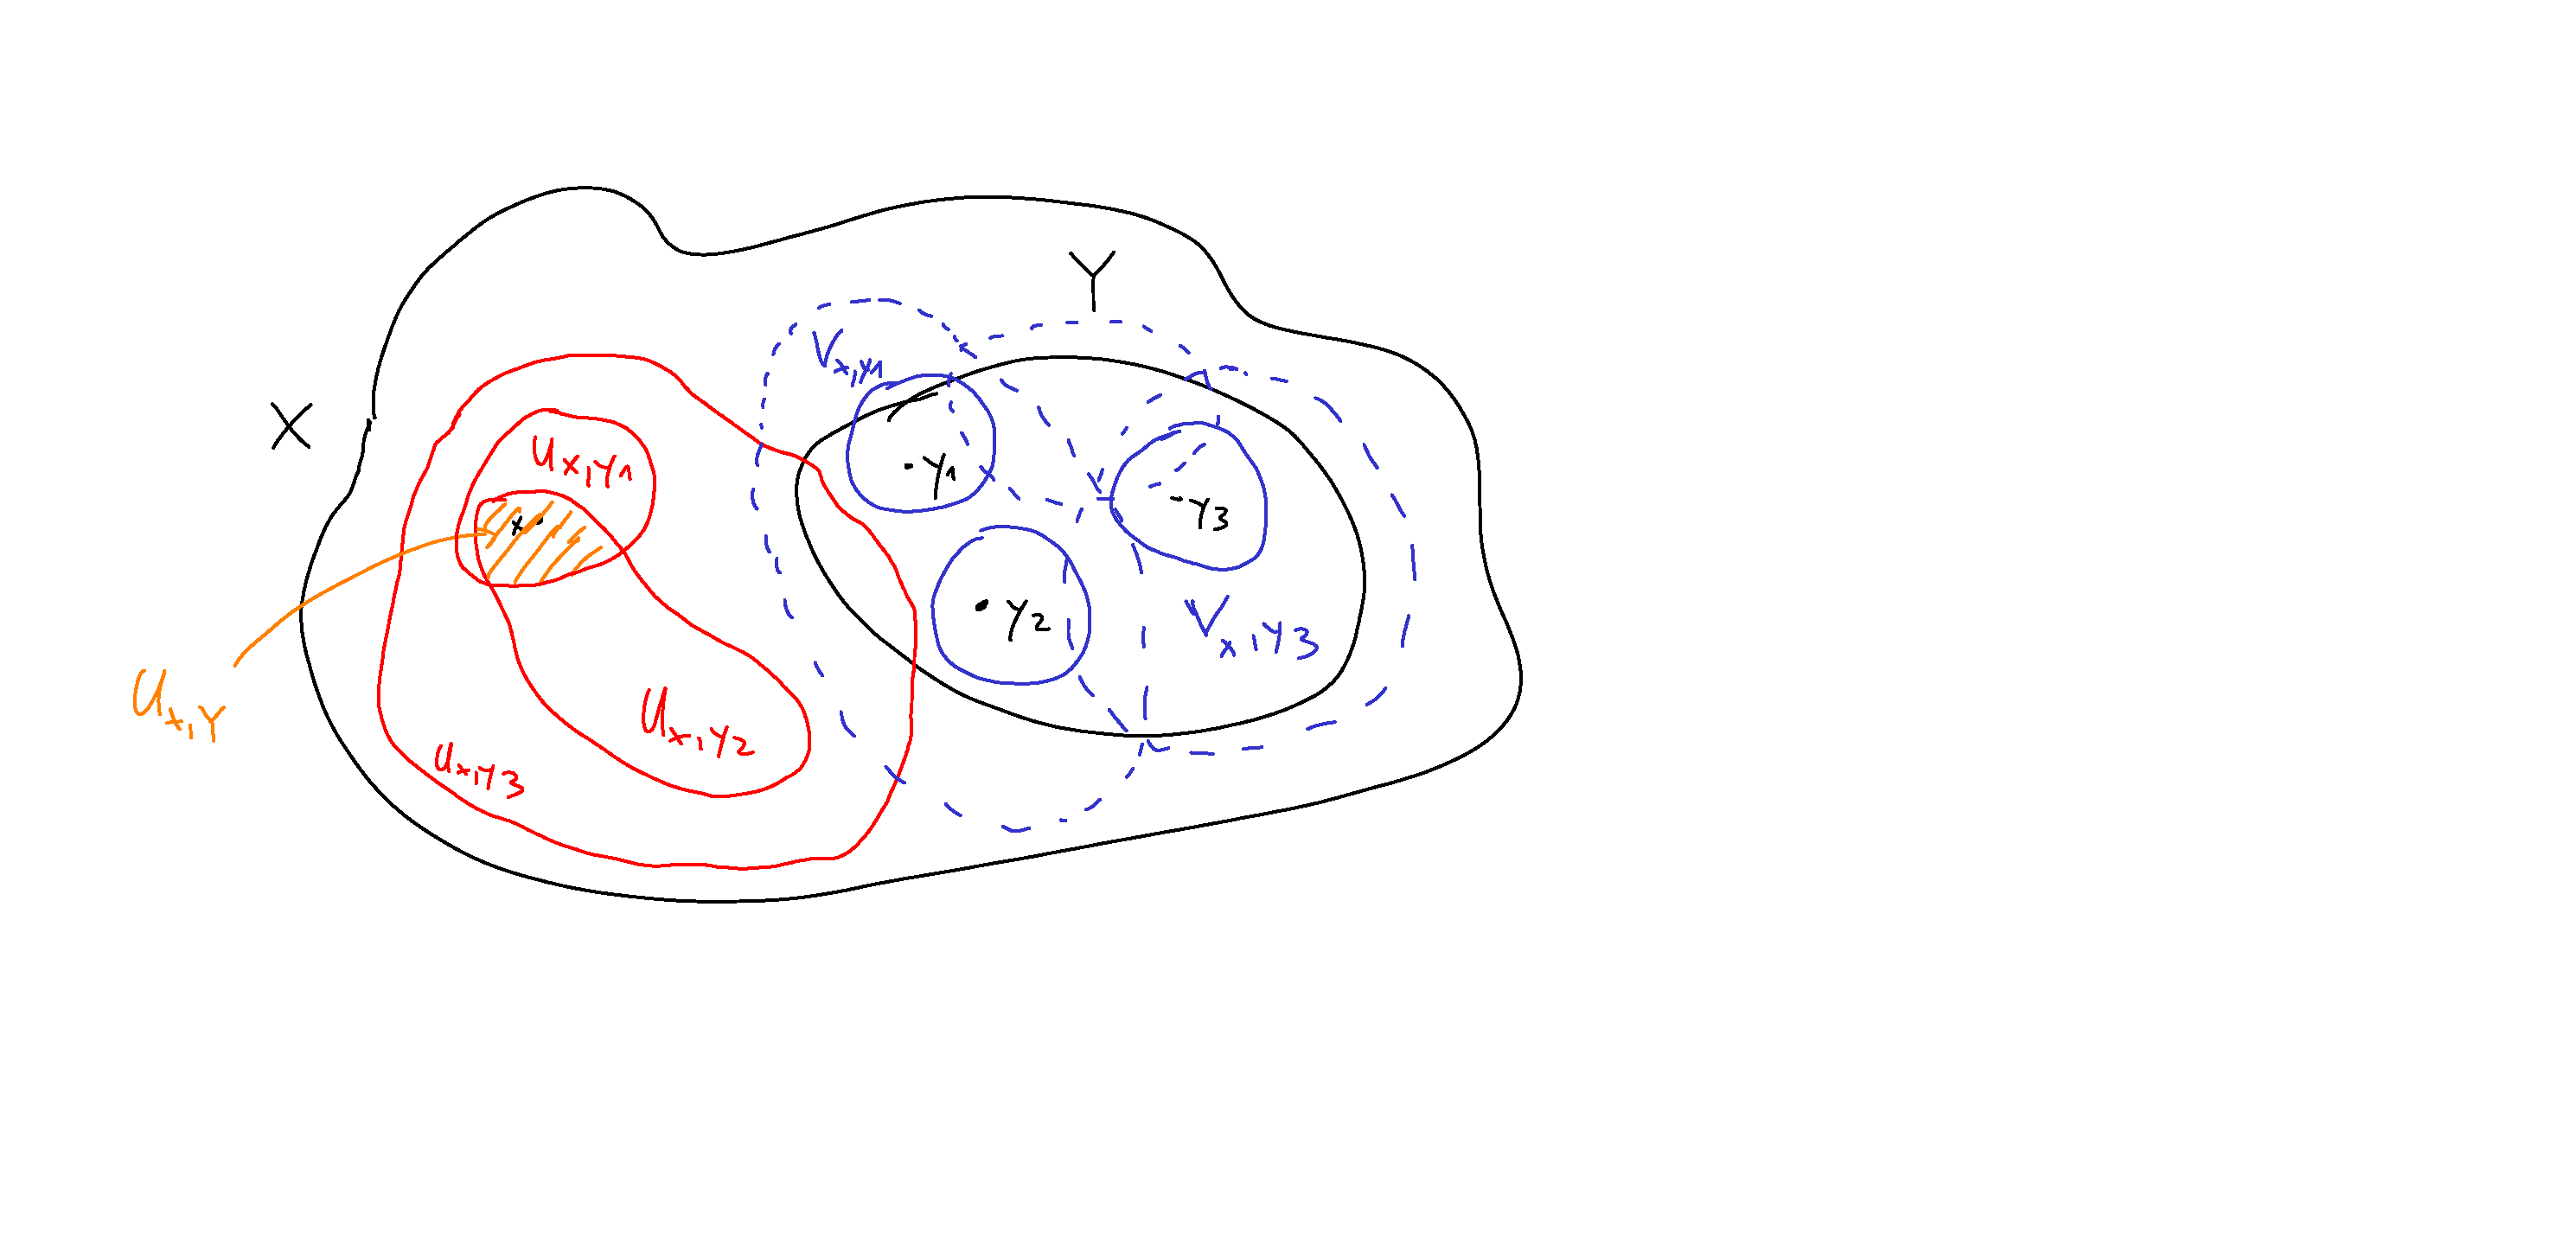
\includegraphics[scale=0.4]{figures/Lemma5.5.pdf}
    \caption{Skizze zum Beweis von Lemma \ref{lm:in-hausdorff-raum-sind-kompakte-mengen-t3}}
\end{figure}
\begin{proof}[Beweis von \autoref{thm:kompakte-menge-in-hausdorff-raum-ist-abgeschlossen}]
    Nach \autoref{lm:in-hausdorff-raum-sind-kompakte-mengen-t3} existieren $\forall x\in X \setminus Y$ ein $U_{x,Y}$ mit $x\in U_{x,Y}$ und $U_{x,Y} \cap Y = \emptyset$. Also ist
    \[
    X \setminus Y = \bigcup_{x\in X \setminus Y} U_{x,Y}
    .\] 
    offen und somit ist $Y$ abgeschlossen.
\end{proof}

\begin{comment}
\begin{example}['Gegenbeispiel' zu Satz \ref{thm:kompakte-menge-in-hausdorff-raum-ist-abgeschlossen}]
    Sei $G$ die \vocab{Gerade mit zwei Urpsrüngen}: \\
    Betrachte  $\R\cup \left \{0'\right\} $ mit $U$ Umgebung von  $a\in \R$ falls $\exists ε>0$ mit $(a-ε, a+ε)\subset U$ und $U$ Umgebung von  $0'$ und  $U$ Umgebung von  $0'$, falls  $\exists ε>0$ mit $(-ε,0 \cup (0,ε) \subset U$ und $0' \in U$. \\
    Wir können uns gewissermaßen  $0,0'$ gleichberechtigt vorstellen, nur dass die beiden Punkte verschieden sind. \\
    Dann ist  $[-1,1] \subset G$ kompakt (Übung!), aber nicht abegschlossen, da $0' \in G \setminus [-1,1]$ ist, dies aber keine Umgebung von $0'$ ist.
    \begin{figure}[H]
        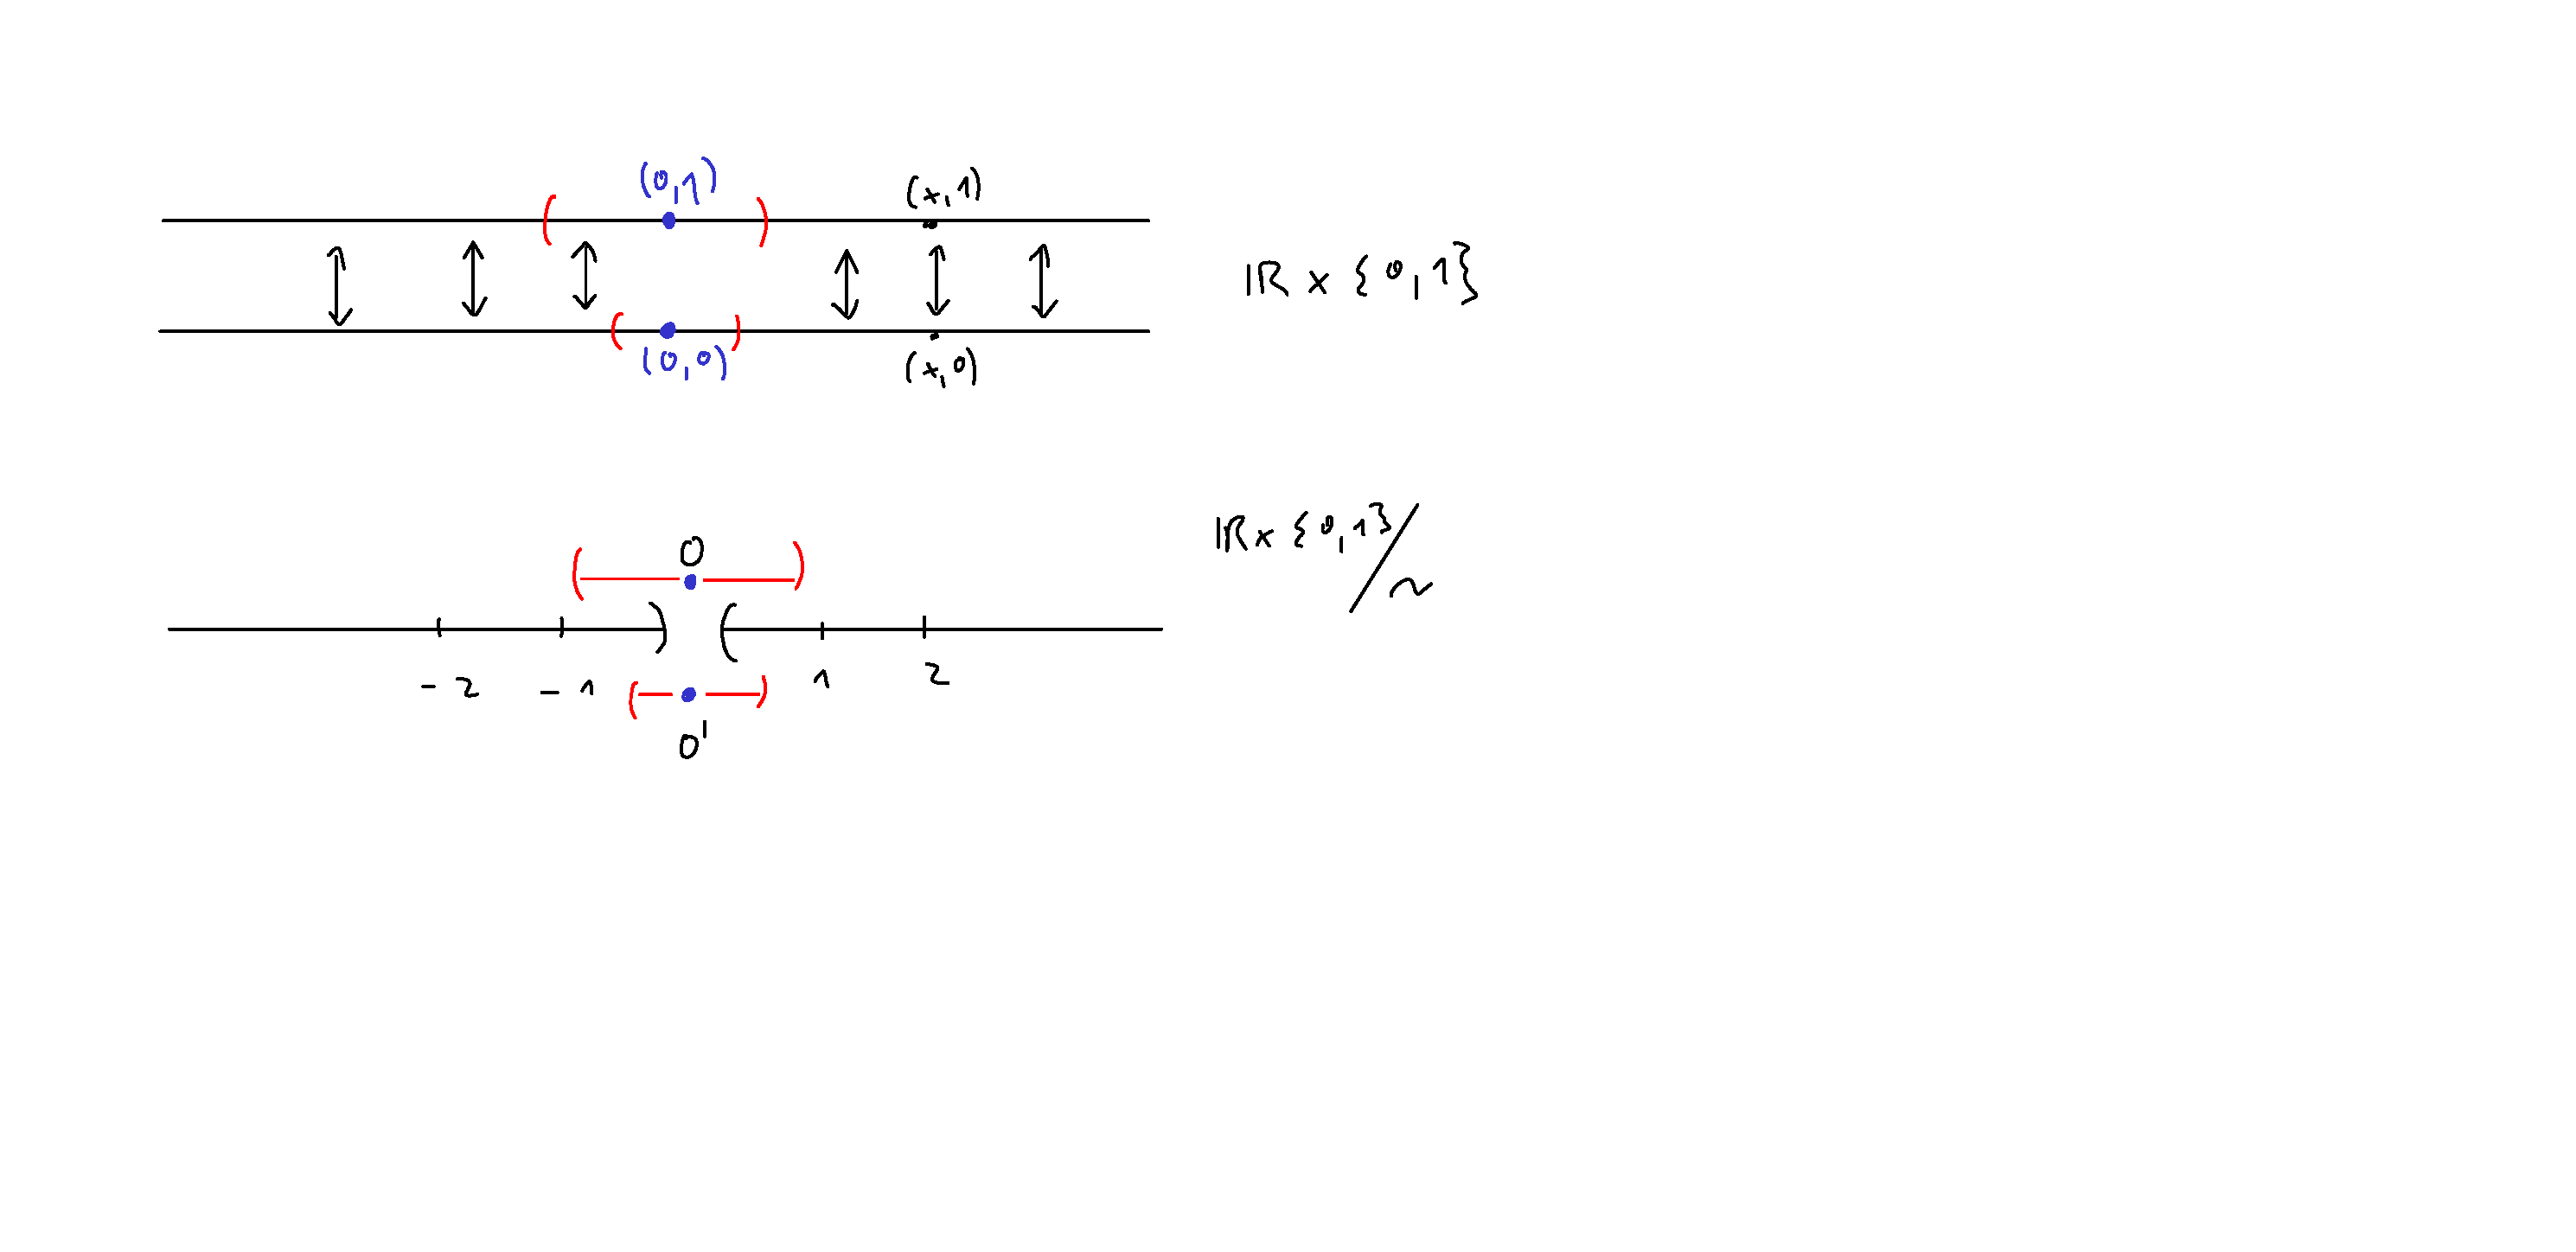
\includegraphics[scale=0.4]{figures/line-with-2-origins.pdf}
    \caption{Gerade mit 2 Ursprüngen}
    \end{figure}
\end{example}
\end{comment}

\begin{example}['Gegenbeispiel' zu Satz \ref{thm:kompakte-menge-in-hausdorff-raum-ist-abgeschlossen}]
    Sei $G$ die \vocab{Gerade mit zwei Urpsrüngen}: \\
    Betrachte $G:=\R \cup  \left \{0'\right\} $ als Menge, und charakterisiere die Umgebungen folgendermaßen:
    \begin{itemize}
        \item Für einen Punkt $a\in \R$, d.h. $a\neq 0'$ ist $U$ eine Umgebung von  $a$ genau dann, wenn  $\exists ε>0$, sodass $(a-ε,a+ε)\subset U$. (das Intervall $(a-ε,a+ε)$ ist hier als Teilmenge von  $\R$ zu verstehen)
        \item Für den Punkt $0'\not\in \R$ ist $U$ eine Umgebung von $a$ genau dann, wenn  $\exists ε>0$ mit $(-ε,0) \cup (0,ε)\subset U$.
    \end{itemize}
    Da offene Mengen genau diejenigen Mengen sind, die Umgebung all ihrer Punkte sind, haben wir damit die offenen Mengen von $G$ charakterisiert. \\
    Wir können uns $G$ vorstellen als  $\R$, in dem der Ursprung durch zwei gleichberechtigte Ursprünge ersetzt worden ist, die beide (bis auf sich selbst) die gleichen Umgebungen besitzen, die aber nicht zwingend gegenseitig in ihren Umgebungen liegen, d.h. nicht 'nah' beieinander sind. \\
    Dann ist $[-1,1]\subset \R\subset G$ kompakt (\autoref{aufgabe-2.3}), wir behaupten, dass $[-1,1]$ jedoch nicht abgeschlossen ist in  $G$. Sonst wäre in der Tat  $G \setminus [-1,1]$ offen, und es ist $0' \in G\setminus [-1,1]$, aber es handelt sich nicht um eine Umgebung von $0'$, weil für kein  $ε$ die Intervalle  $(-ε,0)$ und  $(0,ε)$ in  $G\setminus [-1,1]$ liegen. \\
\end{example}
\begin{dremark}
    Das Beispiel zeigt also, dass wir die Hausdorff-Bedingung in \autoref{thm:kompakte-menge-in-hausdorff-raum-ist-abgeschlossen} nicht fallen lassen können, d.h. es gibt nicht abgeschlossene, kompakte Mengen.
\end{dremark}

\begin{remark*}[Mehr zur Gerade mit 2 Ursprüngen]
    Wir geben zwei weitere (äquivalente) Definitionen der Gerade mit 2 Ursprüngen, um so hoffentlich eine bessere Vorstellung zu ermöglichen:
    \begin{enumerate}[i)]
        \item Setze $G:= \R\setminus \left \{0\right\} \cup \left \{a,b\right\} $ als Mengen. Als Basis wählen wir
            \begin{itemize}
                \item Alle offenen Bälle aus $\R$, die nicht die $0$ enthalten.
                \item Für jedes  $ε>0$ die Menge  $(-ε,0)\cup \left \{a\right\} \cup (0,ε)$
                \item Für jedes $ε>0$ die Menge  $(-ε,0)\cup \left \{b\right\} \cup (0,ε)$
            \end{itemize}
        In diesem Fall können wir Homöomorphismen zu obiger Definition bauen, indem wir $0 \mapsto a$ und  $0' \mapsto b$ wählen, und alle andere Punkte kanonisch 'auf sich selbst' schicken.
    \item  Wir können $G$ auch als Quotientenraum einer Teilmenge von  $\R$ auffassen. Betrachte hierzu $\R\times \left \{0,1\right\} \subset \R^2$ mit der Produkttopologie bzw. mit der Teilraumtopologie von $\R^2$ (diese beiden sind äquivalent, wie man sich leicht überlegt). Es handelt sich also um zwei parallele, voneinander getrennte Geraden. Nun identifizieren wir korrespondierende Punkte beider Geraden miteinander, allerdings nicht deren Ursprüngen. Wir erzeugen also die Äquivalenzrelation $\sim $ generiert durch $(x,0) \sim (x,1)$ für $x\neq 0$ und bilden bezüglich dieser Relation den Quotientenraum. Was wir erhalten, ist genau $G$. Indem wir mit  $G$ definiert wie in der Vorlesung die Abbildung von  $\R\times \left \{0,1\right\}$ nach $G$ definieren durch
         \[
             (a,b) \mapsto \begin{cases}
                 a & \text{falls } a\neq 0 \\
                 0 & \text{falls } (a,b) = (0,0) \\
                 0' & \text{falls } (a,b) = (0,1)
             \end{cases}
        .\]
        sehen wir schnell, dass diese über den Quotientenraum $\R\times \left \{0,1\right\} / \sim $ faktorisiert (universelle Eigenschaft!) und die entstehende Abbildung bijektiv und stetig ist. Dass es sich um einen Homöomorphismus handelt, sei hier nicht nachgerechnet sondern nur angemerkt.
    \end{enumerate}
    \begin{figure}[H]
        \centering
\begin{tikzpicture}
    %Spaces
    %Top space
    \draw[->] (0,3) -- (7,3);
    \fill[blue] (3.5,3) circle (2pt) node[anchor=south] {$0'$};
    \draw[->] (0,2) -- (7,2) ;
    \fill[blue] (3.5,2) circle (2pt) node[anchor=north] {$0$};
    %Bottom space
    \draw[->] (0,0) -- (3.4,0) (3.6,0) -- (7,0);
    \fill[blue] (3.5,-0.5) circle (2pt) node[anchor=north] {$0'$};
    \fill[blue] (3.5,0.5) circle (2pt) node[anchor=south] {$0$};
    %Numbers and gluing arrows
    \foreach \x in {-3,-2,-1,1,2,3} {
        \fill (\x+3.5,3) circle (2pt) node[anchor=south] {$\x'$};
        \fill (\x+3.5,2) circle (2pt) node[anchor=north] {$\x$};
        \fill (\x+3.5,0) circle (2pt) node[anchor=north] {$\x$};
        \draw[<->] (\x+3.5,2.2) -- (\x+3.5, 2.8);
    }
    %Labels
    \node at (8,2.5) {$\R\times \left \{0,1\right\} $};
    \node at (8,0) {$G$};

    %Neighborhoods
    %Top
    \draw[green!40!black,thick] (3,2.9) -- (4,2.9) node[midway,anchor=north] {$U_{0'}$};
    \draw[red,thick] (2.8,2.1) -- (3.7,2.1) node[midway,anchor=south] {$U_{0}$};

    \draw[green!40!black,thick] (3,0.1) -- (3.4,0.1) (3.6,0.1) -- (4,0.1) node[anchor=south west] {$U_{0'}$};
    \fill[green!40!black,thick] (3.5,0.2) circle (2pt);

    \draw[red,thick] (2.8,-0.1) -- (3.4,-0.1) (3.6,-0.1) -- (3.7,-0.1) node[anchor=north west] {$U_{0}$};
    \fill[red,thick] (3.5,-0.2) circle (2pt);

    \draw[->,snake=snake,very thick,orange,segment amplitude = .4mm, segment length=2mm, line after snake =2mm] (1.5,1.5) -- (1.5,0.4);
\end{tikzpicture}
    \caption{Gerade mit 2 Ursprüngen als Quotientenraum von $\R\times \left \{0,1\right\} \subset \R^2$}
    \end{figure}
\end{remark*}



Nun sind wir gewappnet für den
\begin{proof}[Beweis von \autoref{thm:heine-borel} (\nameref{thm:heine-borel})]
    '$2) \implies 1)$'. Sei $X\subset \R^n$ kompakt. Dann ist sie abgeschlossen nach \ref{thm:kompakte-menge-in-hausdorff-raum-ist-abgeschlossen}.
    Zudem ist $X\subset \bigcup_{x\in X} U(x,1)$ eine offene Überdeckung. Da $X$ kompakt finden wir endlich viele  $x_1,\ldots,x_n\in X$ mit
    \[
        X \subset \bigcup_{i=1}^n U(x_i,1)
    .\] 
    Also ist
    \[
        \diam(X) \leq  \max \left \{d(x_i,x_j)\right\} +2 < \infty
    .\] 
    und somit ist $X$ auch beschränkt. \\
    ' $1)\implies 2)$'. Da $X$ beschränkt ist,  $\exists m>0$ mit $X\subset [-m,m]^n\subset \R^n$. Da $X$ abgeschlossen ist, genügt es nach \autoref{thm:abgeschlossene-menge-in-kompaktem-raum-ist-kompakt} zu zeigen, dass  $[-m,m]^n$ kompakt ist. \\
    Wir führen einen Widerspruchsbeweis, nimm also an, dass  $[-m,m]^n$ nicht kompakt ist. Dann existiert eine offene Überdeckung  $\left \{U_i\right\} _{i \in I}$ ohne endliche Teilüberdeckung. \\
    \noindent\begin{minipage}{0.5\textwidth}
    Unterteile $[-m,m]^n$ in  $2^n$ gleich große Unterwürfel (halbiere jede Seite). Mindestens ein Unterwürfel hat keine endliche Teilüberdeckung. Unterteile diesen Würfel weiter und wähle wieder einen Unterwüfel, der keine endliche Teilüberdeckung hat. \\
    Wir erhalten eine Folge von Würfeln
     \[
         [-m,m]^n =     Q_0 \supset Q_1 \supset Q_2 \supset Q_3 \supset \ldots
    .\] 
    die jeweils keine endliche Teilüberdeckung durch $U_i's$ besitzen. \\
    \end{minipage}
    \begin{minipage}{0.5\textwidth}
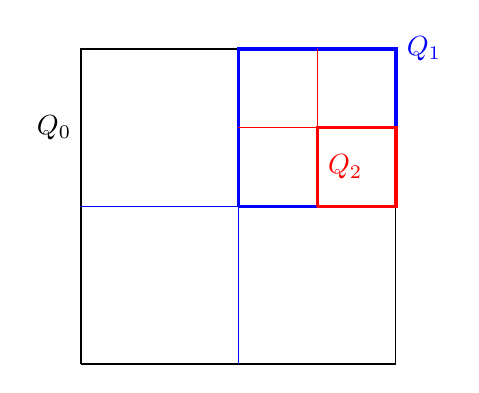
\begin{tikzpicture}
    \draw (-2,-2) -- (-2,2) node[near end, anchor=east]{$Q_0$}-- (2,2) -- (2,-2) -- (-2,-2);
    \draw[blue] (-2,0) -- (2,0);
    \draw[blue] (0,-2) -- (0,2);
    \draw[blue,very thick] (0,0) -- (2,0) -- (2,2) node[anchor=west]{$Q_1$} -- (0,2) -- (0,0) ; 
    \draw[red] (1,0) -- (1,2);
    \draw[red] (0,1) -- (2,1);
    \draw[red, very thick] (1,0) -- (1,1) node[anchor=west, midway]{$Q_2$} -- (2,1) -- (2,0) -- (1,0);
\end{tikzpicture}
    \end{minipage}
    Sei  $x_i \in Q_i$ beliebig. Dann ist $x_i$ eine Cauchy-Folge, also existiert $x = \lim_{i\to \infty} x_i$, und $x\in Q_0$, da $Q_0$ abgeschlossen. \\
    Somit gibt es ein $U_j$ mit  $x\in U_j$, da die $\left \{U_i\right\} _{i \in I}$ eine Überedeckung von $Q_0$ waren. Damit ist auch $U(x,ε) \subset U_j$ für ein $ε>0$. Wähle einen Würfel $x\in Q_k$ mit Kantenlänge $< \frac{ε}{\sqrt{n} }$, dann ist auch $Q_k \subset U(x,ε) \subset U_j$. Das ist aber ein Widerspruch dazu, dass $Q_k$ keine endliche Teilüberdeckung hat, \contra. \\
    Also ist  $Q_0$ kompakt.
\end{proof}



\begin{theorem}[Bilder kompakter Räume]\label{thm:bild-von-kompaktem-raum-ist-kompakt}
    Sei $f: X \to  Y$ stetig und surjektiv und $X$ kompakt. Dann ist auch  $Y$ kompakt. 
\end{theorem}
\begin{proof}
    Sei $\left \{U_i\right\} _{i \in I}$ offene Überdeckung von $Y$. Dann ist
     \[
         \left \{f^{-1}(U_i)\right\} _{i \in I}
    .\] 
    offene Überdeckung von $X$. Da  $X$ kompakt ist, gibt es  $J\subset I$ endlich mit $X = \bigcup_{j\in J} f^{-1}(U_j)$. Dann ist 
    \[
        Y = f(X) = \bigcup_{j\in J} f(f^{-1}(U_j)) = \bigcup_{j\in J} U_j
    .\] 
    Also existiert eine endliche Teilüberdeckung von $Y$.
\end{proof}
\begin{corollary}\label{cor:stetige-abbildung-von-kompaktem-raum-in-hausdorff-raum-ist-abgeschlossen}
    Sei $f: X \to  Y$ stetig, $X$ kompakt und  $Y$ Hausdorff. Dann ist  $f$ abgeschlossen, d.h. $\forall A\subset X$ abgeschlossen ist $f(A) \subset Y$ abgeschlossen.
\end{corollary}
\begin{proof}
    Sei $A\subset X$ abgeschlossen. Dann ist $A$ kompakt nach \autoref{thm:kompakte-menge-in-hausdorff-raum-ist-abgeschlossen}, also ist  $f(A)$ kompakt nach \autoref{thm:bild-von-kompaktem-raum-ist-kompakt} (weil $f: X \to f(A)\subset Y$ surjektiv ist). Damit ist dann $f(A)$ abegschlossen nach \autoref{thm:kompakte-menge-in-hausdorff-raum-ist-abgeschlossen}. \\
    Also sind Bilder abgeschlossener Mengen abgeschlossen.
\end{proof}

\begin{corollary}[Homöomorphismen]\label{cor:stetige-bijektion-von-kompaktem-raum-in-hausdorff-raum-ist-homöomorphismus}
    Ist $f: X \to  Y$ stetig und bijektiv, $X$ kompakt und  $Y$ Hausdorff, dann ist  $f$ ein Homöomorphismus.
\end{corollary}

\begin{proof}
    Wir müssen zeigen, dass die Umkehrabbildung stetig ist. Dafür reicht es zu zeigen, dass $\forall A\subset X$ abgeschlossen auch $f(A) = (f^{-1})^{-1}(A)$ abgeschlossen ist. Das gilt aber genau nach vorherigem \autoref{cor:stetige-abbildung-von-kompaktem-raum-in-hausdorff-raum-ist-abgeschlossen}
\end{proof}
\begin{corollary}\label{cor:abbildung-von-kompaktem-raum-in-hausdorff-raum-ist-quotientenabbildung}
    Sei $f: X \to  Y$ stetig und surjektiv, $X$ kompakt und  $Y$ Hausdorffsch. Dann trägt  $Y$ die Quotiententopologie, d.h.  $U\subset Y$ offen genau dann, wenn $f^{-1}(U) \subset X$ offen.
\end{corollary}

\begin{proof}
    '$\implies$' folgt wegen Stetigkeit. \\
    '$\impliedby$' Ist $f^{-1}(U) \subset X$ offen, dann ist $f^{-1}(Y \setminus U ) = X \setminus f^{-1}(U)$ abgeschlossen in $X$, also folgt aus dem \autoref{cor:stetige-abbildung-von-kompaktem-raum-in-hausdorff-raum-ist-abgeschlossen}
     \[
         Y \setminus U \stackrel{\text{surj.}}{=}   f\left( \underbrace{f^{-1}\left( Y \setminus U \right)}_{\text{abgeschlossen}}  \right) 
    .\] 
    abgeschlossen ist, also ist $U\subset Y$ offen.
\end{proof}
Kommen wir nun zum
\begin{proof}[Beweis von \autoref{thm:kreis-ist-quotientenraum-von-einheitsintervall} (Fortsetzung)]
    Schon gezeigt:
        \begin{equation*}
        \begin{array}{c c l} 
            [0,1] & \longrightarrow & S_1 \\
        t & \longmapsto &  2^{2\pi it}
        \end{array}
    \end{equation*}
    ist stetig und surjektiv und faktorisiert über
    \[
        [0,1] /\left \{0,1\right\}  \to  S^1
    .\] 
    mit $f$ stetig und bijektiv. Wir wissen nun:  $S^1$ ist Hausdorffsch und  $[0,1]$ ist kompakt. Nach \autoref{thm:bild-von-kompaktem-raum-ist-kompakt} ist auch  $[0,1] /\left \{0,1\right\} $ kompakt, also ist $f$ ein Homöomorphismus nach \autoref{cor:stetige-bijektion-von-kompaktem-raum-in-hausdorff-raum-ist-homöomorphismus}
\end{proof}


\begin{theorem}\label{thm:kompakter-hausdorff-raum-ist-normal}
    Jeder kompakte Hausdorff-Raum ist normal.
\end{theorem}
\begin{proof}
    Seien $A,B\subset X$ abgeschlossen und disjunkt. Da $X$ kompakt ist, sind  $A,B$ kompakt. Nach Lemma 5.5 existieren  $\forall a\in A$ offene Mengen $U_a, V_a$ mit $a\in U_a, B\subset V_a$ und $U_a \cap V_a = \emptyset$. Dann ist
    \[
    A \subset \bigcup_{a\in A} U_a
    .\] 
    Also existieren $a_1,\ldots,a_n\in A$ mit
    \[
    A\subset \bigcup_{i=1}^n U_{a_i}
    .\] 
    wegen $A$ kompakt. Setze nun
    \[
    U_A := \bigcup_{i=1}^n U_{a_i}\supset A \qquad U_B := \bigcap_{i=1}^n V_{a_i}\supset B
    .\] 
$\forall i$ ist 
\[
    U_{a_i} \cap U_B \subset U_{a_i} \cap V_{a_i} = \emptyset
.\] 
und daraus folgt, dass
\[
U_A \cap U_B = \emptyset
.\] 
\end{proof}

\begin{theorem}[Quotientenräume von Hausdorffräumen]\label{thm:quotientenraum-von-hausdorffraum-ist-hausdorff-gdw-projektion-abgeschlossen}
    Sei $X$ kompakt und Hausdorffsch, $q: X \to  Z$ surjektiv, wobei  $Z$ die Quotiententopologie trage. Dann sind äquivalent: 
    \begin{enumerate}[1)]
        \item $Z$ ist Hausdorffsch
        \item  $q$ ist abgeschlossen
    \end{enumerate}
\end{theorem}
\begin{proof}
    Die Richtung '$1) \implies 2)$' ist genau \autoref{cor:stetige-abbildung-von-kompaktem-raum-in-hausdorff-raum-ist-abgeschlossen} \\
    '$2)\implies_1)$': Jedes $z\in Z$ hat ein Urbild $x\in X$ unter $q$. Es ist  $\left \{x\right\} \subset X$ abgeschlossen, da $X$ hausdorffsch. Wegen  $q$ abgeschlossen folgt nun, dass auch
    \[
        \left \{z\right\}  = q(\left \{x\right\} )
    .\] 
    abgeschlossen ist. \\
    \begin{ddefinition}[saturierte Menge]\label{def:saturierte-menge}
    Wir nennen Teilmenge $W\subset X$ heißt \vocab[Menge!saturiert]{saturiert}, falls $W = q^{-1}(q(W))$ (insbesondere sind alle Urbilder saturiert, und $\iff  \forall x\in X \setminus W : g(x) \in Z \setminus g(W)$).
    \end{ddefinition}
\begin{remark}
    Sei $U\subset X$ offen und saturiert, dann ist $q(U)$ offen. Hierzu schreibe
    \[
        U = q^{-1}(q(U)) \implies q(U) \text{ offen}
    .\] 
\end{remark}
Seien $y\neq z\in Z$. Dann sind $\left \{y\right\} ,\left \{z\right\} $ abgeschlossen und disjunkt. Dann sind auch
\[
    A = q^{-1}(y) \qquad B = q^{-1}(z)
.\] 
abgeschlossen und disjunkt (in  $X$). Nach Annahme ist  $X$ kompakt und Hausdorff, also normal nach Satz \ref{thm:kompakter-hausdorff-raum-ist-normal}. Also existieren  $U_1,U_2\subset X$ offen mit $A\subset U_1,B\subset U_2$ und $U_1 \cap U_2 = \emptyset$. Setze
\[
    V_1 := X \setminus q^{-1}(q(X\setminus U_1)) \qquad V_2 := X \setminus q^{-1}(q(X\setminus U_2))
.\] 
\begin{claim}
    Es sind $V_1,V_2$ offen, disjunkt und saturiert und $A\subset V_1$ sowie $B\subset V_2$.
\end{claim}
\begin{subproof}
    Nächstes Mal.
\end{subproof}
Es folgt, dass $q(V_1),q(V_2)$ offen in $Z$ sind. Weiter ist  $y\in q(A)\subset q(V_1)$ und $z\in q(B) \subset q(V_2)$. Da $V_1,V_2$ disjunkt und saturiert, sind auch $q(V_1),q(V_2)$ disjunkt und wir sind fertig.
\end{proof}
